\begin{figure}
\centering

\begin{subfigure}[t]{0.16\textwidth}
\centering
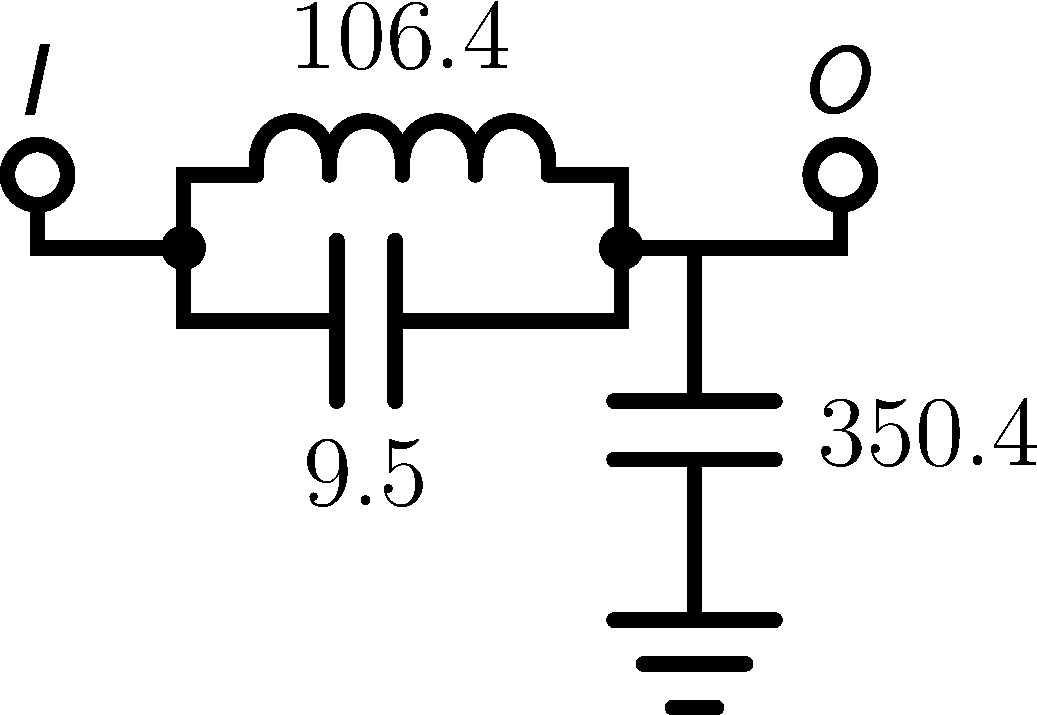
\includegraphics[scale = 0.14]{../ch6/figures/lpf1_circuit1}
\caption{\label{fig:lpf1_circuita}}
\end{subfigure}%
\begin{subfigure}[t]{0.16\textwidth}
\centering
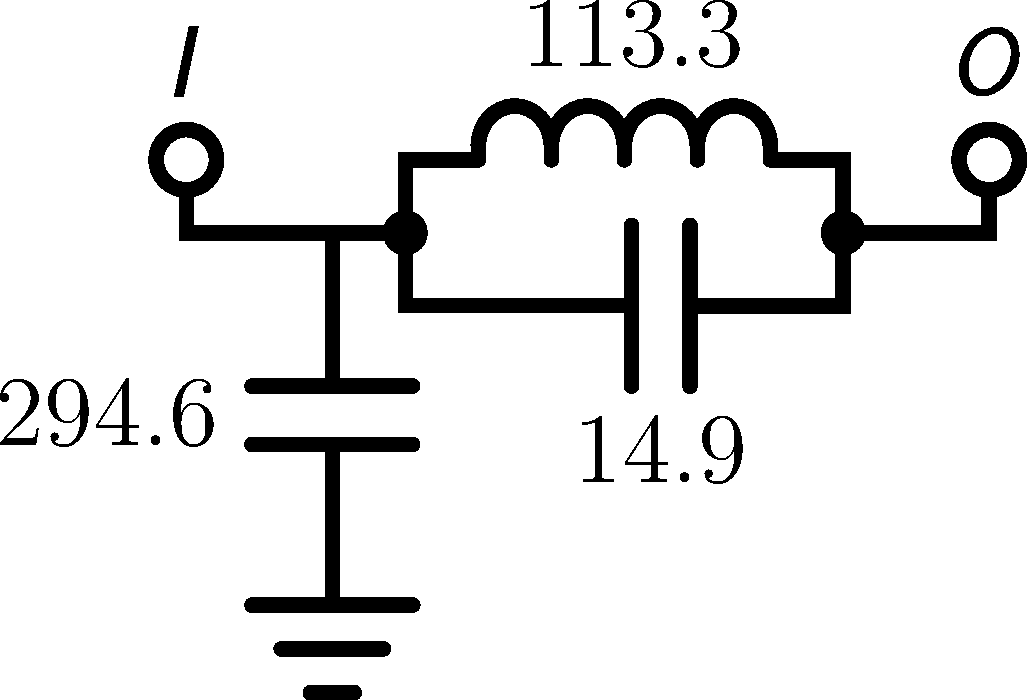
\includegraphics[scale = 0.14]{../ch6/figures/lpf1_circuit2}
\caption{\label{fig:lpf1_circuitb}}
\end{subfigure}%
\begin{subfigure}[t]{0.16\textwidth}
\centering
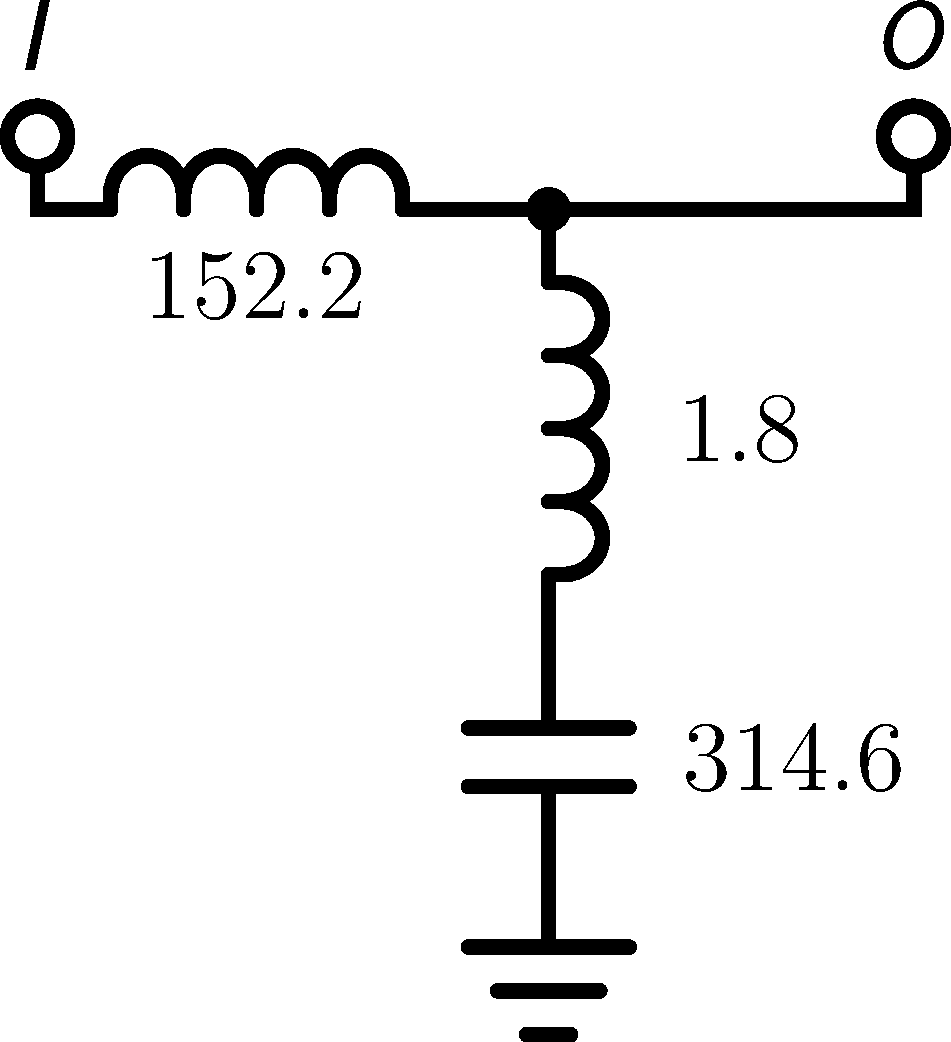
\includegraphics[scale = 0.14]{../ch6/figures/lpf1_circuit4}
\caption{\label{fig:lpf1_circuitc}}
\end{subfigure}%
\begin{subfigure}[t]{0.16\textwidth}
\centering
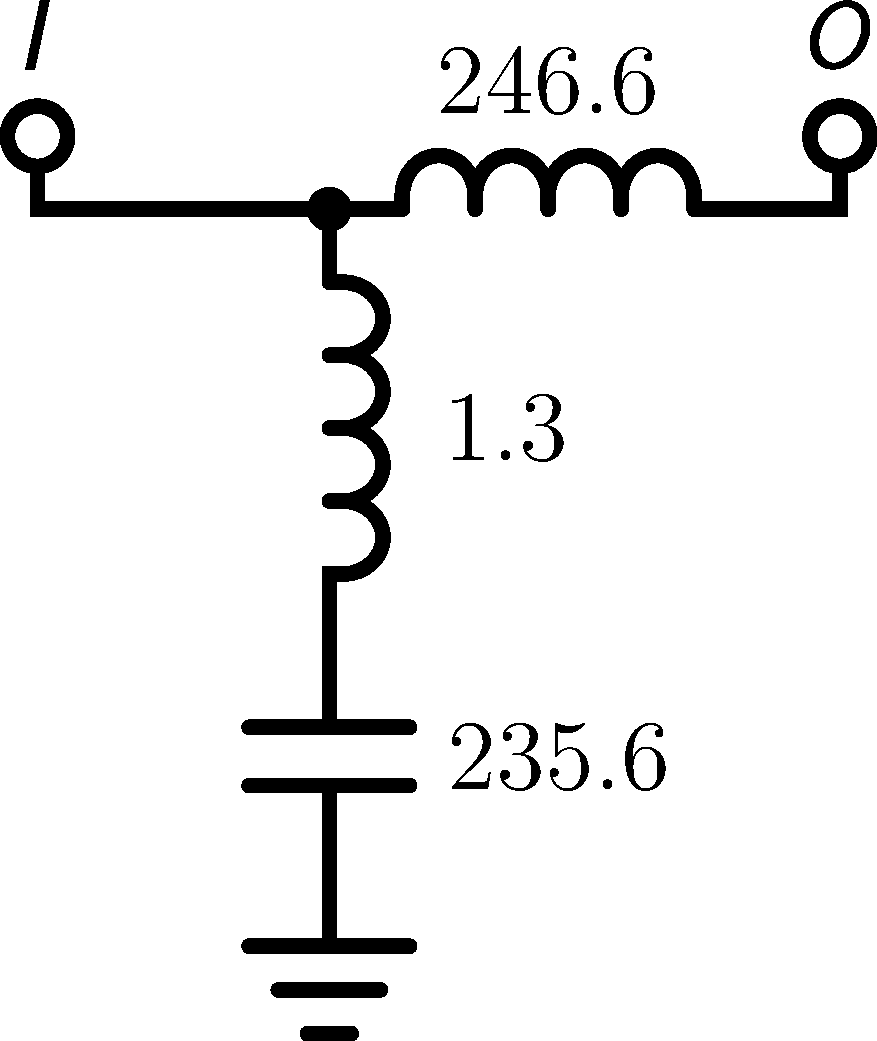
\includegraphics[scale = 0.14]{../ch6/figures/lpf1_circuit5}
\caption{\label{fig:lpf1_circuitd}}
\end{subfigure}%
\begin{subfigure}[t]{0.16\textwidth}
\centering
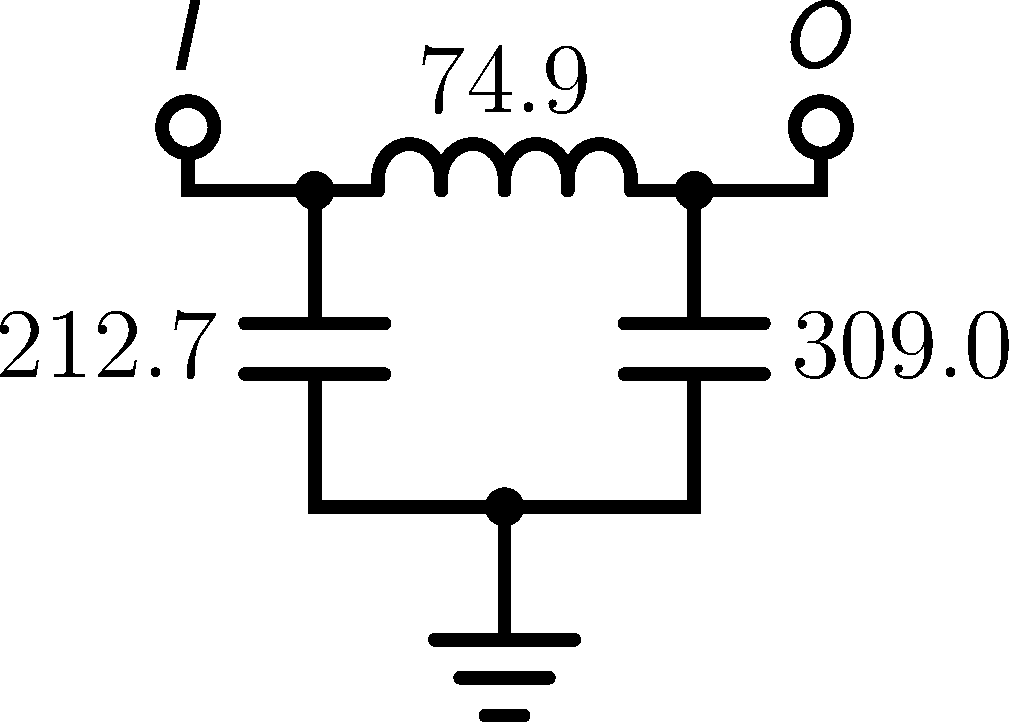
\includegraphics[scale = 0.14]{../ch6/figures/lpf1_circuit3}
\caption{\label{fig:lpf1_circuite}}
\end{subfigure}%
\begin{subfigure}[t]{0.16\textwidth}
\centering
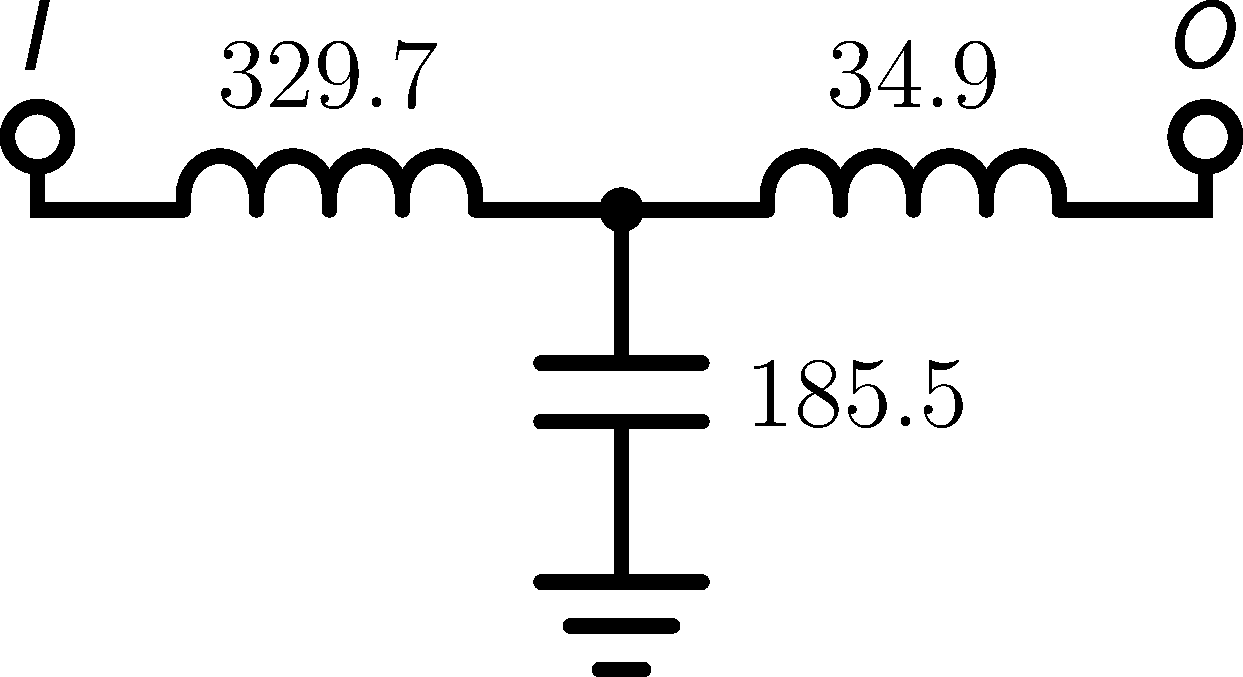
\includegraphics[scale = 0.14]{../ch6/figures/lpf1_circuit6}
\caption{\label{fig:lpf1_circuitf}}
\end{subfigure}%
\vspace{0.06in}
\begin{subfigure}[t]{\textwidth}
\centering
% 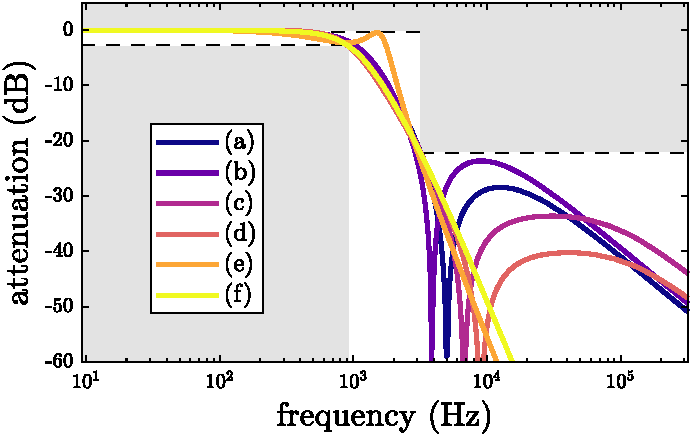
\includegraphics[width=\textwidth]{../ch6/figures/lpf1_magnitude}
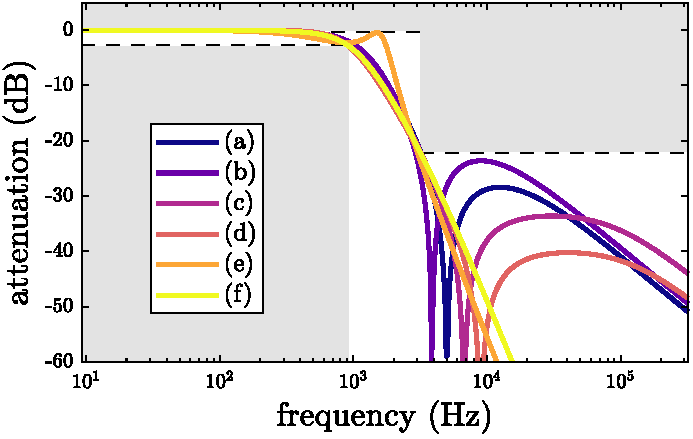
\includegraphics[width=0.5\textwidth]{../ch6/figures/reduced/r_lpf1_magnitude}
\caption{\label{fig:lpf1_magnitude}}
\end{subfigure}%

\caption[All feasible, minimum complexity circuits and attenuation responses for \nameref{sec:ch6:lpf} task \#1.]{All feasible, minimum complexity circuits and attenuation responses for \nameref{sec:ch6:lpf} task \#1 (units are mH and nF).\label{fig:lpf1}}

\end{figure}